\documentclass[]{article}
\usepackage{lmodern}
\usepackage{amssymb,amsmath}
\usepackage{ifxetex,ifluatex}
\usepackage{fixltx2e} % provides \textsubscript
\ifnum 0\ifxetex 1\fi\ifluatex 1\fi=0 % if pdftex
  \usepackage[T1]{fontenc}
  \usepackage[utf8]{inputenc}
\else % if luatex or xelatex
  \ifxetex
    \usepackage{mathspec}
  \else
    \usepackage{fontspec}
  \fi
  \defaultfontfeatures{Ligatures=TeX,Scale=MatchLowercase}
\fi
% use upquote if available, for straight quotes in verbatim environments
\IfFileExists{upquote.sty}{\usepackage{upquote}}{}
% use microtype if available
\IfFileExists{microtype.sty}{%
\usepackage{microtype}
\UseMicrotypeSet[protrusion]{basicmath} % disable protrusion for tt fonts
}{}
\usepackage[margin=1in]{geometry}
\usepackage{hyperref}
\hypersetup{unicode=true,
            pdftitle={R Notebook},
            pdfborder={0 0 0},
            breaklinks=true}
\urlstyle{same}  % don't use monospace font for urls
\usepackage{color}
\usepackage{fancyvrb}
\newcommand{\VerbBar}{|}
\newcommand{\VERB}{\Verb[commandchars=\\\{\}]}
\DefineVerbatimEnvironment{Highlighting}{Verbatim}{commandchars=\\\{\}}
% Add ',fontsize=\small' for more characters per line
\usepackage{framed}
\definecolor{shadecolor}{RGB}{248,248,248}
\newenvironment{Shaded}{\begin{snugshade}}{\end{snugshade}}
\newcommand{\KeywordTok}[1]{\textcolor[rgb]{0.13,0.29,0.53}{\textbf{#1}}}
\newcommand{\DataTypeTok}[1]{\textcolor[rgb]{0.13,0.29,0.53}{#1}}
\newcommand{\DecValTok}[1]{\textcolor[rgb]{0.00,0.00,0.81}{#1}}
\newcommand{\BaseNTok}[1]{\textcolor[rgb]{0.00,0.00,0.81}{#1}}
\newcommand{\FloatTok}[1]{\textcolor[rgb]{0.00,0.00,0.81}{#1}}
\newcommand{\ConstantTok}[1]{\textcolor[rgb]{0.00,0.00,0.00}{#1}}
\newcommand{\CharTok}[1]{\textcolor[rgb]{0.31,0.60,0.02}{#1}}
\newcommand{\SpecialCharTok}[1]{\textcolor[rgb]{0.00,0.00,0.00}{#1}}
\newcommand{\StringTok}[1]{\textcolor[rgb]{0.31,0.60,0.02}{#1}}
\newcommand{\VerbatimStringTok}[1]{\textcolor[rgb]{0.31,0.60,0.02}{#1}}
\newcommand{\SpecialStringTok}[1]{\textcolor[rgb]{0.31,0.60,0.02}{#1}}
\newcommand{\ImportTok}[1]{#1}
\newcommand{\CommentTok}[1]{\textcolor[rgb]{0.56,0.35,0.01}{\textit{#1}}}
\newcommand{\DocumentationTok}[1]{\textcolor[rgb]{0.56,0.35,0.01}{\textbf{\textit{#1}}}}
\newcommand{\AnnotationTok}[1]{\textcolor[rgb]{0.56,0.35,0.01}{\textbf{\textit{#1}}}}
\newcommand{\CommentVarTok}[1]{\textcolor[rgb]{0.56,0.35,0.01}{\textbf{\textit{#1}}}}
\newcommand{\OtherTok}[1]{\textcolor[rgb]{0.56,0.35,0.01}{#1}}
\newcommand{\FunctionTok}[1]{\textcolor[rgb]{0.00,0.00,0.00}{#1}}
\newcommand{\VariableTok}[1]{\textcolor[rgb]{0.00,0.00,0.00}{#1}}
\newcommand{\ControlFlowTok}[1]{\textcolor[rgb]{0.13,0.29,0.53}{\textbf{#1}}}
\newcommand{\OperatorTok}[1]{\textcolor[rgb]{0.81,0.36,0.00}{\textbf{#1}}}
\newcommand{\BuiltInTok}[1]{#1}
\newcommand{\ExtensionTok}[1]{#1}
\newcommand{\PreprocessorTok}[1]{\textcolor[rgb]{0.56,0.35,0.01}{\textit{#1}}}
\newcommand{\AttributeTok}[1]{\textcolor[rgb]{0.77,0.63,0.00}{#1}}
\newcommand{\RegionMarkerTok}[1]{#1}
\newcommand{\InformationTok}[1]{\textcolor[rgb]{0.56,0.35,0.01}{\textbf{\textit{#1}}}}
\newcommand{\WarningTok}[1]{\textcolor[rgb]{0.56,0.35,0.01}{\textbf{\textit{#1}}}}
\newcommand{\AlertTok}[1]{\textcolor[rgb]{0.94,0.16,0.16}{#1}}
\newcommand{\ErrorTok}[1]{\textcolor[rgb]{0.64,0.00,0.00}{\textbf{#1}}}
\newcommand{\NormalTok}[1]{#1}
\usepackage{graphicx,grffile}
\makeatletter
\def\maxwidth{\ifdim\Gin@nat@width>\linewidth\linewidth\else\Gin@nat@width\fi}
\def\maxheight{\ifdim\Gin@nat@height>\textheight\textheight\else\Gin@nat@height\fi}
\makeatother
% Scale images if necessary, so that they will not overflow the page
% margins by default, and it is still possible to overwrite the defaults
% using explicit options in \includegraphics[width, height, ...]{}
\setkeys{Gin}{width=\maxwidth,height=\maxheight,keepaspectratio}
\IfFileExists{parskip.sty}{%
\usepackage{parskip}
}{% else
\setlength{\parindent}{0pt}
\setlength{\parskip}{6pt plus 2pt minus 1pt}
}
\setlength{\emergencystretch}{3em}  % prevent overfull lines
\providecommand{\tightlist}{%
  \setlength{\itemsep}{0pt}\setlength{\parskip}{0pt}}
\setcounter{secnumdepth}{0}
% Redefines (sub)paragraphs to behave more like sections
\ifx\paragraph\undefined\else
\let\oldparagraph\paragraph
\renewcommand{\paragraph}[1]{\oldparagraph{#1}\mbox{}}
\fi
\ifx\subparagraph\undefined\else
\let\oldsubparagraph\subparagraph
\renewcommand{\subparagraph}[1]{\oldsubparagraph{#1}\mbox{}}
\fi

%%% Use protect on footnotes to avoid problems with footnotes in titles
\let\rmarkdownfootnote\footnote%
\def\footnote{\protect\rmarkdownfootnote}

%%% Change title format to be more compact
\usepackage{titling}

% Create subtitle command for use in maketitle
\providecommand{\subtitle}[1]{
  \posttitle{
    \begin{center}\large#1\end{center}
    }
}

\setlength{\droptitle}{-2em}

  \title{R Notebook}
    \pretitle{\vspace{\droptitle}\centering\huge}
  \posttitle{\par}
    \author{}
    \preauthor{}\postauthor{}
    \date{}
    \predate{}\postdate{}
  

\begin{document}
\maketitle

\begin{Shaded}
\begin{Highlighting}[]
\NormalTok{diamonds <-}\StringTok{ }\KeywordTok{read.delim}\NormalTok{(}\StringTok{"HW-diamonds.txt"}\NormalTok{, }\DataTypeTok{header =} \OtherTok{FALSE}\NormalTok{, }\DataTypeTok{sep =} \StringTok{""}\NormalTok{, }\DataTypeTok{dec =} \StringTok{"."}\NormalTok{)}
\end{Highlighting}
\end{Shaded}

\begin{Shaded}
\begin{Highlighting}[]
\KeywordTok{head}\NormalTok{(diamonds)}
\end{Highlighting}
\end{Shaded}

\begin{verbatim}
##     V1 V2   V3  V4   V5
## 1 0.30  D  VS2 GIA 1302
## 2 0.30  E  VS1 GIA 1510
## 3 0.30  G VVS1 GIA 1510
## 4 0.30  G  VS1 GIA 1260
## 5 0.31  D  VS1 GIA 1641
## 6 0.31  E  VS1 GIA 1555
\end{verbatim}

\begin{Shaded}
\begin{Highlighting}[]
\KeywordTok{colnames}\NormalTok{(diamonds) <-}\StringTok{ }\KeywordTok{c}\NormalTok{(}\StringTok{"caratage"}\NormalTok{, }\StringTok{"purity"}\NormalTok{, }\StringTok{"clarity"}\NormalTok{, }\StringTok{"certificate"}\NormalTok{, }\StringTok{"price"}\NormalTok{)}
\NormalTok{diamonds}\OperatorTok{$}\NormalTok{purity <-}\StringTok{ }\KeywordTok{factor}\NormalTok{(diamonds}\OperatorTok{$}\NormalTok{purity, }\DataTypeTok{levels=}\KeywordTok{c}\NormalTok{(}\StringTok{"D"}\NormalTok{, }\StringTok{"E"}\NormalTok{, }\StringTok{"F"}\NormalTok{, }\StringTok{"G"}\NormalTok{, }\StringTok{"H"}\NormalTok{, }\StringTok{"I"}\NormalTok{))}
\NormalTok{diamonds}\OperatorTok{$}\NormalTok{clarity <-}\StringTok{ }\KeywordTok{factor}\NormalTok{(diamonds}\OperatorTok{$}\NormalTok{clarity, }\DataTypeTok{levels=}\KeywordTok{c}\NormalTok{(}\StringTok{"VS2"}\NormalTok{, }\StringTok{"VS1"}\NormalTok{, }\StringTok{"VVS2"}\NormalTok{, }\StringTok{"VVS1"}\NormalTok{, }\StringTok{"IF"}\NormalTok{))}
\end{Highlighting}
\end{Shaded}

\begin{Shaded}
\begin{Highlighting}[]
\KeywordTok{summary}\NormalTok{(diamonds)}
\end{Highlighting}
\end{Shaded}

\begin{verbatim}
##     caratage      purity clarity   certificate     price      
##  Min.   :0.1800   D:16   VS2 :53   GIA:151     Min.   :  638  
##  1st Qu.:0.3500   E:44   VS1 :81   HRD: 79     1st Qu.: 1625  
##  Median :0.6200   F:82   VVS2:78   IGI: 78     Median : 4215  
##  Mean   :0.6309   G:65   VVS1:52               Mean   : 5019  
##  3rd Qu.:0.8500   H:61   IF  :44               3rd Qu.: 7446  
##  Max.   :1.1000   I:40                         Max.   :16008
\end{verbatim}

\begin{Shaded}
\begin{Highlighting}[]
\KeywordTok{library}\NormalTok{(ggplot2)}
\end{Highlighting}
\end{Shaded}

\begin{verbatim}
## Warning: package 'ggplot2' was built under R version 3.5.3
\end{verbatim}

\begin{verbatim}
## 
## Attaching package: 'ggplot2'
\end{verbatim}

\begin{verbatim}
## The following object is masked _by_ '.GlobalEnv':
## 
##     diamonds
\end{verbatim}

\subsubsection{1. Plot price vs caratage and log(price) vs caratage.
Decide on which response variable is better to
use}\label{plot-price-vs-caratage-and-logprice-vs-caratage.-decide-on-which-response-variable-is-better-to-use}

\begin{Shaded}
\begin{Highlighting}[]
\KeywordTok{ggplot}\NormalTok{(}\DataTypeTok{data=}\NormalTok{diamonds, }\KeywordTok{aes}\NormalTok{(price, caratage)) }\OperatorTok{+}\StringTok{ }
\StringTok{        }\KeywordTok{geom_point}\NormalTok{()}
\end{Highlighting}
\end{Shaded}

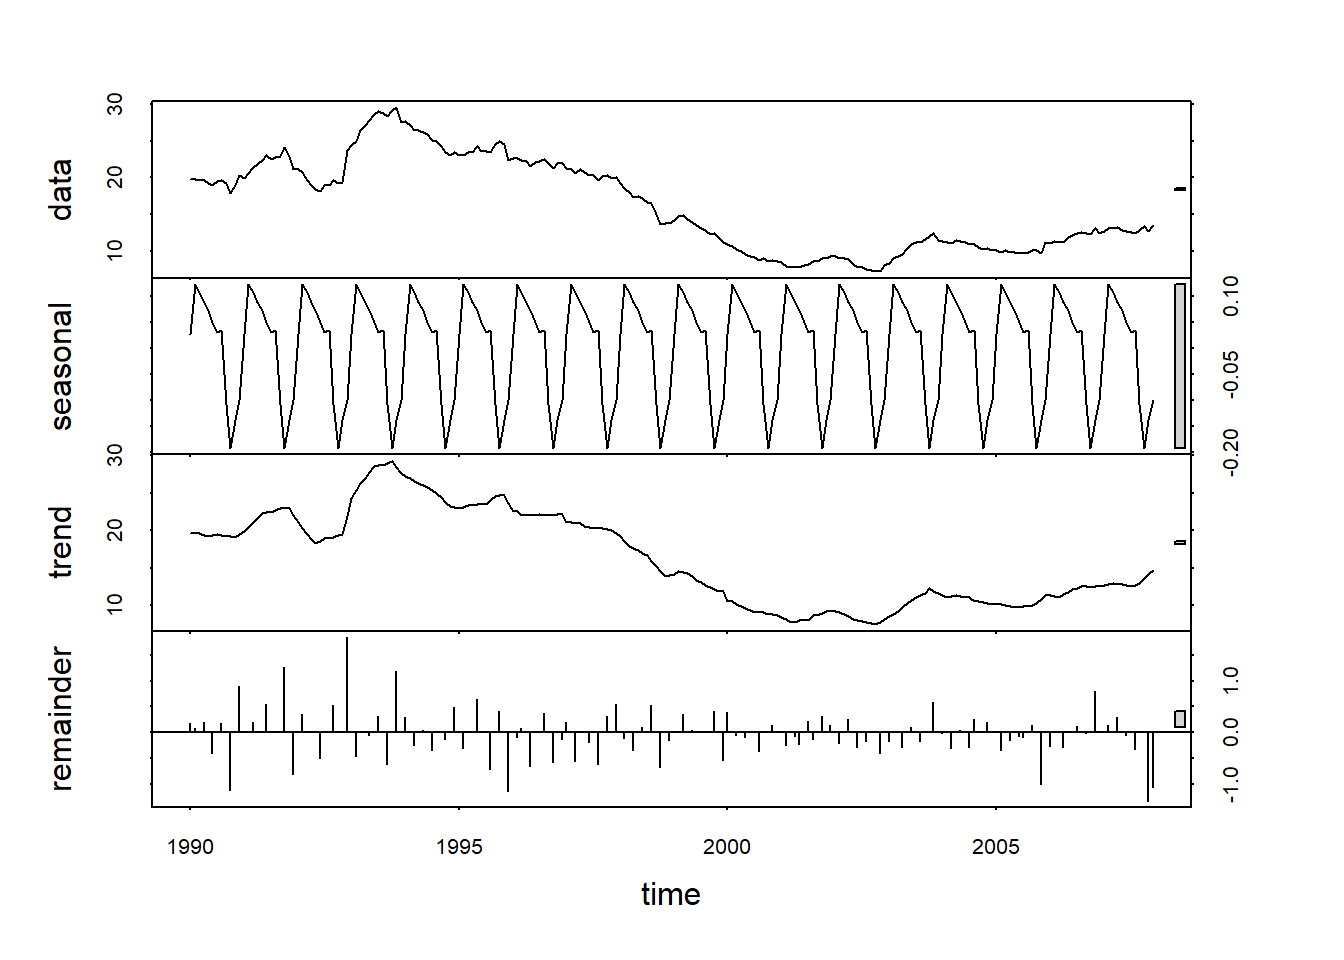
\includegraphics{nacho_analysis_files/figure-latex/unnamed-chunk-6-1.pdf}

\begin{Shaded}
\begin{Highlighting}[]
\KeywordTok{ggplot}\NormalTok{(}\DataTypeTok{data=}\NormalTok{diamonds, }\KeywordTok{aes}\NormalTok{(}\KeywordTok{log}\NormalTok{(price), caratage)) }\OperatorTok{+}\StringTok{ }
\StringTok{        }\KeywordTok{geom_point}\NormalTok{()}
\end{Highlighting}
\end{Shaded}

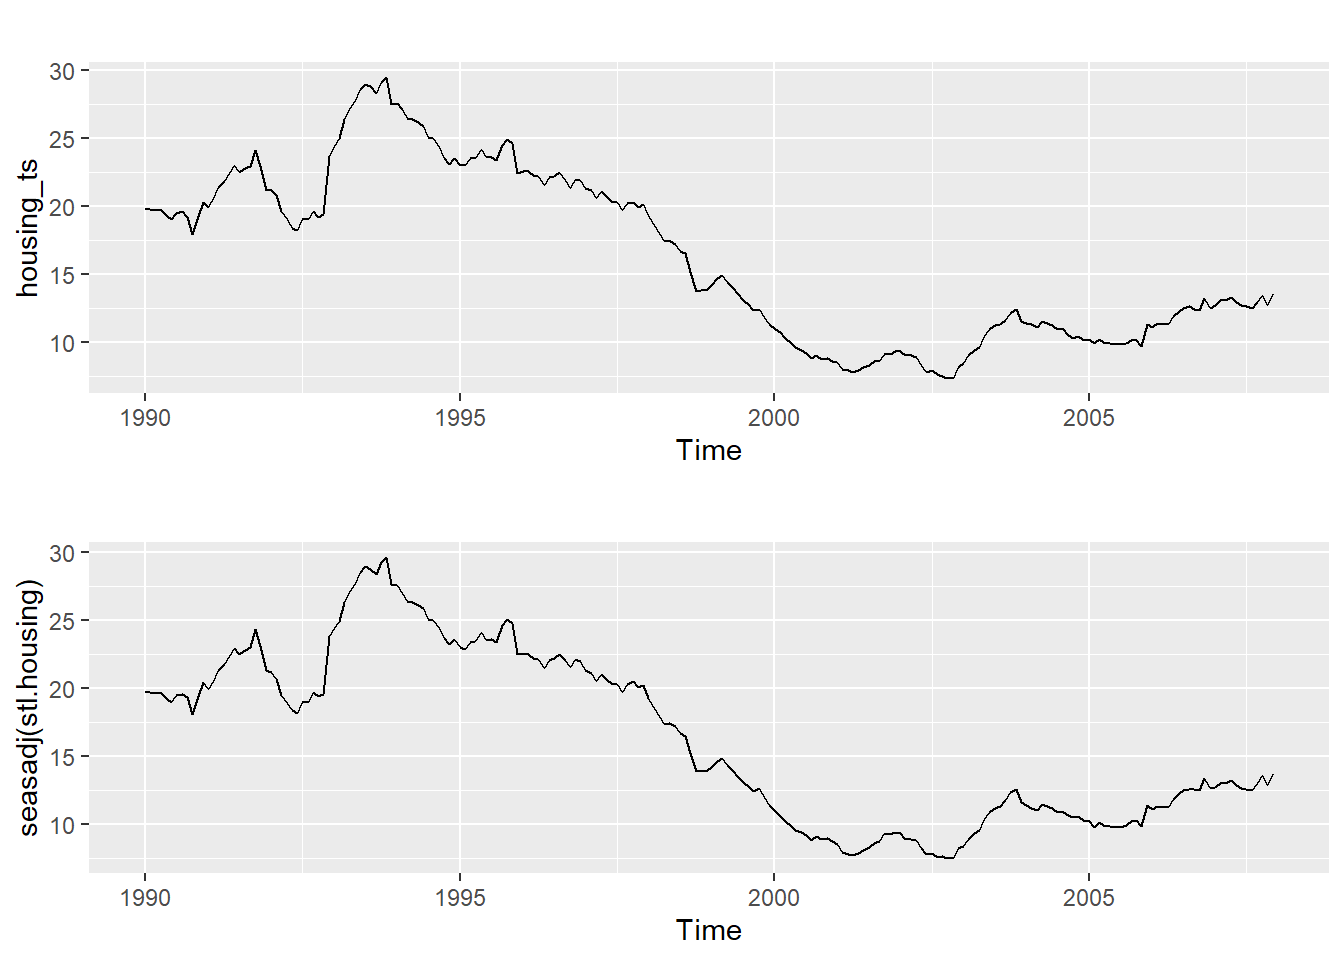
\includegraphics{nacho_analysis_files/figure-latex/unnamed-chunk-6-2.pdf}

log(price) seems more linear (maybe different transformations?)

\subsubsection{2. Find a suitable way to include, besides caratage, the
other categorical
information}\label{find-a-suitable-way-to-include-besides-caratage-the-other-categorical-information}

available: clarity, color and certificate. Use the worst level of each
categorical variable as the reference category and HRD for certification
institution. Comment on the model fitted, and perform a basic analysis
of the residuals (normality, constant variance, independence, you may
also want to use the function outlierTest or residualPlot ).

\begin{Shaded}
\begin{Highlighting}[]
\CommentTok{#Starting model}
\NormalTok{model1.}\DecValTok{1}\NormalTok{<-}\KeywordTok{lm}\NormalTok{(}\DataTypeTok{formula =}\NormalTok{ price }\OperatorTok{~}\StringTok{ }\NormalTok{caratage }\OperatorTok{+}\StringTok{ }\NormalTok{purity }\OperatorTok{+}\StringTok{ }\NormalTok{clarity }\OperatorTok{+}\StringTok{ }\NormalTok{certificate, }\DataTypeTok{data =}\NormalTok{ diamonds)}
\KeywordTok{summary}\NormalTok{(model1.}\DecValTok{1}\NormalTok{)}
\end{Highlighting}
\end{Shaded}

\begin{verbatim}
## 
## Call:
## lm(formula = price ~ caratage + purity + clarity + certificate, 
##     data = diamonds)
## 
## Residuals:
##     Min      1Q  Median      3Q     Max 
## -1740.0  -428.8  -128.3   314.3  3634.1 
## 
## Coefficients:
##                Estimate Std. Error t value Pr(>|t|)    
## (Intercept)    -1622.83     247.65  -6.553 2.51e-10 ***
## caratage       12766.40     190.02  67.183  < 2e-16 ***
## purityE        -1439.09     207.98  -6.919 2.83e-11 ***
## purityF        -1841.69     195.23  -9.433  < 2e-16 ***
## purityG        -2176.67     200.39 -10.862  < 2e-16 ***
## purityH        -2747.15     202.91 -13.538  < 2e-16 ***
## purityI        -3313.10     212.71 -15.575  < 2e-16 ***
## clarityVS1       317.44     128.09   2.478   0.0138 *  
## clarityVVS2      600.85     130.28   4.612 5.95e-06 ***
## clarityVVS1     1102.72     144.45   7.634 3.18e-13 ***
## clarityIF       1792.01     171.19  10.468  < 2e-16 ***
## certificateHRD    15.23     107.25   0.142   0.8872    
## certificateIGI   141.26     128.26   1.101   0.2716    
## ---
## Signif. codes:  0 '***' 0.001 '**' 0.01 '*' 0.05 '.' 0.1 ' ' 1
## 
## Residual standard error: 710.4 on 295 degrees of freedom
## Multiple R-squared:  0.9581, Adjusted R-squared:  0.9564 
## F-statistic: 562.5 on 12 and 295 DF,  p-value: < 2.2e-16
\end{verbatim}

\begin{Shaded}
\begin{Highlighting}[]
\CommentTok{#Let's try to predict log(price)}
\NormalTok{model1.}\DecValTok{2}\NormalTok{<-}\KeywordTok{lm}\NormalTok{(}\DataTypeTok{formula =} \KeywordTok{log}\NormalTok{(price) }\OperatorTok{~}\StringTok{ }\NormalTok{caratage }\OperatorTok{+}\StringTok{ }\NormalTok{purity }\OperatorTok{+}\StringTok{ }\NormalTok{clarity }\OperatorTok{+}\StringTok{ }\NormalTok{certificate, }\DataTypeTok{data =}\NormalTok{ diamonds)}
\KeywordTok{summary}\NormalTok{(model1.}\DecValTok{2}\NormalTok{)}
\end{Highlighting}
\end{Shaded}

\begin{verbatim}
## 
## Call:
## lm(formula = log(price) ~ caratage + purity + clarity + certificate, 
##     data = diamonds)
## 
## Residuals:
##      Min       1Q   Median       3Q      Max 
## -0.31236 -0.11520  0.01613  0.10833  0.36339 
## 
## Coefficients:
##                 Estimate Std. Error t value Pr(>|t|)    
## (Intercept)     6.502651   0.048178 134.971  < 2e-16 ***
## caratage        2.855013   0.036968  77.230  < 2e-16 ***
## purityE        -0.029509   0.040461  -0.729  0.46638    
## purityF        -0.106358   0.037981  -2.800  0.00544 ** 
## purityG        -0.206349   0.038985  -5.293 2.35e-07 ***
## purityH        -0.287876   0.039475  -7.293 2.81e-12 ***
## purityI        -0.416557   0.041382 -10.066  < 2e-16 ***
## clarityVS1      0.096609   0.024919   3.877  0.00013 ***
## clarityVVS2     0.201923   0.025344   7.967 3.56e-14 ***
## clarityVVS1     0.297835   0.028102  10.598  < 2e-16 ***
## clarityIF       0.298541   0.033303   8.964  < 2e-16 ***
## certificateHRD -0.008856   0.020864  -0.424  0.67155    
## certificateIGI -0.182711   0.024952  -7.323 2.33e-12 ***
## ---
## Signif. codes:  0 '***' 0.001 '**' 0.01 '*' 0.05 '.' 0.1 ' ' 1
## 
## Residual standard error: 0.1382 on 295 degrees of freedom
## Multiple R-squared:  0.9723, Adjusted R-squared:  0.9712 
## F-statistic: 863.6 on 12 and 295 DF,  p-value: < 2.2e-16
\end{verbatim}

\begin{Shaded}
\begin{Highlighting}[]
\CommentTok{#model1.2 has a lower residual standard error and a higher R^2. We will predict log(price).}

\CommentTok{#By default, the category that R chooses to be the reference or baseline, is the first category that appears alphabetically or  numerically (if categories are coded using 0,1,2,...).}
\CommentTok{#Let's use the worst level of each categorical variable as the reference category and HRD for certification institution.}
\NormalTok{diamonds}\OperatorTok{$}\NormalTok{purity <-}\StringTok{ }\KeywordTok{relevel}\NormalTok{(diamonds}\OperatorTok{$}\NormalTok{purity, }\DataTypeTok{ref =} \StringTok{"I"}\NormalTok{)}
\NormalTok{diamonds}\OperatorTok{$}\NormalTok{clarity <-}\StringTok{ }\KeywordTok{relevel}\NormalTok{(diamonds}\OperatorTok{$}\NormalTok{clarity, }\DataTypeTok{ref =} \StringTok{"VS2"}\NormalTok{)}
\NormalTok{diamonds}\OperatorTok{$}\NormalTok{certificate <-}\StringTok{ }\KeywordTok{relevel}\NormalTok{(diamonds}\OperatorTok{$}\NormalTok{certificate, }\DataTypeTok{ref =} \StringTok{"HRD"}\NormalTok{)}
\NormalTok{model1.}\DecValTok{3}\NormalTok{<-}\KeywordTok{lm}\NormalTok{(}\DataTypeTok{formula =} \KeywordTok{log}\NormalTok{(price) }\OperatorTok{~}\StringTok{ }\NormalTok{caratage }\OperatorTok{+}\StringTok{ }\NormalTok{purity }\OperatorTok{+}\StringTok{ }\NormalTok{clarity }\OperatorTok{+}\StringTok{ }\NormalTok{certificate, }\DataTypeTok{data =}\NormalTok{ diamonds)}
\KeywordTok{summary}\NormalTok{(model1.}\DecValTok{3}\NormalTok{)}
\end{Highlighting}
\end{Shaded}

\begin{verbatim}
## 
## Call:
## lm(formula = log(price) ~ caratage + purity + clarity + certificate, 
##     data = diamonds)
## 
## Residuals:
##      Min       1Q   Median       3Q      Max 
## -0.31236 -0.11520  0.01613  0.10833  0.36339 
## 
## Coefficients:
##                 Estimate Std. Error t value Pr(>|t|)    
## (Intercept)     6.077239   0.048091 126.369  < 2e-16 ***
## caratage        2.855013   0.036968  77.230  < 2e-16 ***
## purityD         0.416557   0.041382  10.066  < 2e-16 ***
## purityE         0.387047   0.030824  12.557  < 2e-16 ***
## purityF         0.310198   0.027479  11.288  < 2e-16 ***
## purityG         0.210207   0.028359   7.412 1.32e-12 ***
## purityH         0.128681   0.028523   4.511 9.31e-06 ***
## clarityVS1      0.096609   0.024919   3.877  0.00013 ***
## clarityVVS2     0.201923   0.025344   7.967 3.56e-14 ***
## clarityVVS1     0.297835   0.028102  10.598  < 2e-16 ***
## clarityIF       0.298541   0.033303   8.964  < 2e-16 ***
## certificateGIA  0.008856   0.020864   0.424  0.67155    
## certificateIGI -0.173855   0.028673  -6.063 4.07e-09 ***
## ---
## Signif. codes:  0 '***' 0.001 '**' 0.01 '*' 0.05 '.' 0.1 ' ' 1
## 
## Residual standard error: 0.1382 on 295 degrees of freedom
## Multiple R-squared:  0.9723, Adjusted R-squared:  0.9712 
## F-statistic: 863.6 on 12 and 295 DF,  p-value: < 2.2e-16
\end{verbatim}

\begin{Shaded}
\begin{Highlighting}[]
\CommentTok{#Same statistics as model1.2.}

\CommentTok{#}
\end{Highlighting}
\end{Shaded}

\subsubsection{3. Try two different remedial
actions:}\label{try-two-different-remedial-actions}

\subsubsection{3a. Create a new categorical variable to segregate the
stones according to caratage: let's say less than 0.5 carats small, 0.5
to less than 1 carat (medium) and 1 carat and over (large). Make small
as the reference category. Add this new variable to the existing model
as well as an interaction term between this new variable and
caratage.}\label{a.-create-a-new-categorical-variable-to-segregate-the-stones-according-to-caratage-lets-say-less-than-0.5-carats-small-0.5-to-less-than-1-carat-medium-and-1-carat-and-over-large.-make-small-as-the-reference-category.-add-this-new-variable-to-the-existing-model-as-well-as-an-interaction-term-between-this-new-variable-and-caratage.}

\begin{itemize}
\item
  Is this regression model satisfactory? Are the standard assumptions of
  linear regression validated? Are the numerical estimates sensible?
\item
  Interpret the interaction parameter med*carat. What can we infer on
  the incremental pricing of caratage in the 3 clusters?
\item
  Which is more highly valued: colour or clarity?
\item
  All other things being equal, what is the average price difference
  between a grade D diamond and another one graded (a) I (b) E?
\item
  All other things being equal, are there price differences amongst the
  stones appraised by the GIA, IGI and HRD?
\end{itemize}

\subsubsection{3b. Include the square of carat as a new explanatory
variable. It avoids the subjectivity of clusters
definition.}\label{b.-include-the-square-of-carat-as-a-new-explanatory-variable.-it-avoids-the-subjectivity-of-clusters-definition.}

\subsubsection{4. Which of the two remedial actions do you prefer and
why? Think on terms of interpretability and validity of the
assumptions.}\label{which-of-the-two-remedial-actions-do-you-prefer-and-why-think-on-terms-of-interpretability-and-validity-of-the-assumptions.}


\end{document}
